 \documentclass{beamer}

%\usefonttheme{professionalfonts} % using non standard fonts for beamer
%\usefonttheme{serif} % default family is serif
%\usepackage{fontspec}
%\setmainfont{Liberation Serif}

\mode<presentation> {
\usetheme{Malmoe} 
\usecolortheme{beaver} 
}

\usepackage{graphicx} 
\usepackage{booktabs} 
\usepackage{amsmath}
\usepackage{graphicx}
\usepackage[colorinlistoftodos]{todonotes}
\usepackage{hyperref}
\usepackage{multimedia}
\usepackage{media9}
\usepackage{tikz}
\usepackage{amsmath}
\usetikzlibrary{calc,positioning}
\usepackage{xcolor}
\usepackage{calrsfs}
\usepackage[utf8]{inputenc}
\usepackage{boondox-calo}
	   %\usepackage{boondox-cal}
       %\usepackage{dutchcal}
       %\usepackage{bickham}
\usepackage{algorithm}
\usepackage{algorithmic}
%\usepackage[noend]{algpseudocode}
\hypersetup{
    colorlinks=true,       
    linkcolor=blue,          
    citecolor=blue,        
    urlcolor=blue           
}
%-----------------------------------------------------------------------
%	TITLE PAGE
%----------------------------------------------------------------------------------------

\title[CPS]{\textcolor{black}{{Cooperative Mobile Manipulation without Explicit Communication \cite{p1}}}} 
\subtitle[]{}

\author{George Kontoudis}
\institute[VT] 
{
AOE5984 Cyber-Physical Systems \& Distributed Control\\
Spring 2017\\
\medskip
\it{Mechanical Engineering Department, Virginia Tech} 
}
\date{\today}

\setbeamertemplate{footline}[text line]{%
  \parbox{\linewidth}{\vspace*{-8pt}\today 
  \hfill\insertshortsubtitle
  \hfill\insertpagenumber}}
\setbeamertemplate{navigation symbols}{}

\begin{document}

\begin{frame}[plain]
\titlepage 
\end{frame}

\begin{frame}
\scriptsize{\frametitle{Outline} }
\tableofcontents 
\end{frame}


%----------------------------------------------------------------------------------------
%	PRESENTATION SLIDES
%----------------------------------------------------------------------------------------

%------------------------------------------------
\section{Motivation}
%------------------------------------------------

\begin{frame}
\frametitle{Motivation}
Communication networks of robots confronts various problems
\begin{enumerate}
\item Very noisy 
\item Demands high computational power
\item Deals with uncertainty 
\item Might get vanished \vspace{.4cm}
\end{enumerate}

Instead, we employ affordable sensing information 
\begin{itemize}
\item Motion planning imposed by the leader
\item Utilize force feedback
\item Information attained locally
\end{itemize}
\end{frame}
%------------------------------------------------
\begin{frame}
\frametitle{Applications}
Both large and small number of robots can be used depending on the object's size

\begin{itemize}
\item Automated construction site\vspace{.3cm}
\item Manufacturing facilities\vspace{.3cm}
\item Structured environment
\end{itemize}
\end{frame}



%------------------------------------------------
\section{Rigid Body Dynamics}
%------------------------------------------------
\subsection{Translational Dynamics}
\begin{frame}
\frametitle{Translational Object Dynamics}
Translational motion subject to Newton's second law
\begin{equation}
M\dot{v}=\sum_{i=1}^N F_i-\mu_{k}Mg\frac{v}{||v||}-\mu_v v
\end{equation}
\begin{itemize}
\item $\mu_k$ coefficient of kinetic friction  \vspace{0.2cm}
\item $\mu_v$ coefficient of rolling friction  \vspace{0.2cm}
\item $\frac{v}{||v||}$ unity tangent vector
\end{itemize}
\end{frame}

%------------------------------------------------
\begin{frame}
\frametitle{Friction}

\begin{columns}[c] 
\column{.56\textwidth}
\begin{itemize}
\item Friction of rigid bodies discriminates in 2 regions \vspace{0.2cm}
\item Static proportional to force \vspace{0.2cm}
\item Kinetic friction assumed constant \vspace{0.2cm}
\item Spinning wheels can replace kinetic w/ viscous friction - velocity related
\end{itemize}

\column{.54\textwidth} 
\centering
 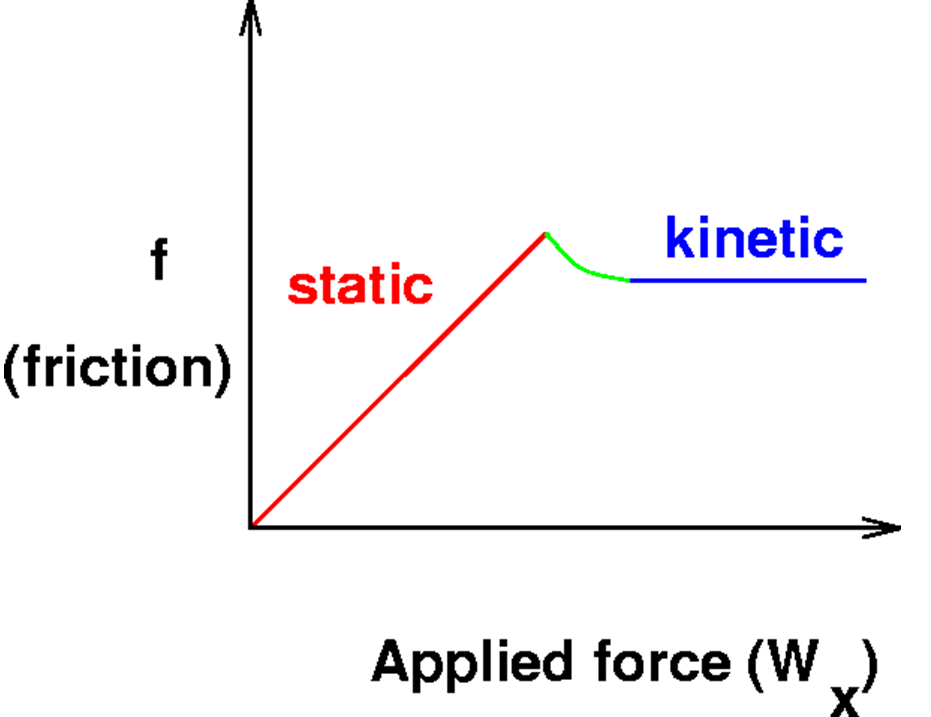
\includegraphics[width=.8\textwidth]{figures/Static_Vs_Kinetic.png}\\
\scriptsize{Source: \url{http://deutsch.physics.ucsc.edu/6A/book/forces/node21.html}}
\end{columns}

\end{frame}

%------------------------------------------------
\begin{frame}
\frametitle{Translational Dynamics Cases}
\begin{enumerate}
\item For lightweight objects after Euler's discretization
\begin{equation}\label{dod}
M\frac{v_{t+1}-v_t}{\Delta t}=\sum_{i=1}^N F_i(t)-\mu_kMg\frac{v_t}{||v_t||}
\end{equation}
\item For heavyweight objects
\begin{equation}\label{roldyn}
M\dot{v}=\sum_{i=1}^N F_i-\mu_v v
\end{equation}
\end{enumerate}
\textbf{Assumption 1:} $M$, $\mu_k$, $\mu_v$, $g$, $N$ given
\end{frame}



%------------------------------------------------
\subsection{Rotational Dynamics}
\begin{frame}
\frametitle{Object's Rotational Dynamics}
\begin{equation}\label{rotDyn1}
J\dot{\omega}=T_1 +\sum_{i=2}^{N}r_i\times F_i-T_f=T_1 +\sum_{i=2}^{N}r_i\times F_i-\frac{\mu_{\nu}}{M}J\omega
\end{equation}
\begin{itemize}
\item $T_f$, static friction related torque, obect's motion $Q \in \mathbb{R}^2$
\item $\sum_{i=2}^{N}r_i\times F_i$, follower robots torque 
\item $r_i$, vector from object's CoM to the contact point 
\item $T_l$, leader's applied torque\vspace{.3cm}
\end{itemize}
\textbf{Assumption 2: }Leader know object's $\omega$ and applies $T_1$
\end{frame}

%------------------------------------------------
\section{Constant Boost Force CB-ANTS}
%------------------------------------------------
\subsection{CB-ANTS Global}
\begin{frame}
\frametitle{CB-ANTS Case}
Constant Boost force (CB-ANTS) case deals with dragging the object \vspace{.3cm}
\begin{itemize}
\item Lightweight objects\vspace{.3cm}
\item Dominant friction is kinetic\vspace{.3cm}
\item Both global and local information studies
\end{itemize}
\end{frame}

%------------------------------------------------

\begin{frame}
\frametitle{CB-ANTS Follower's Controller}
Follower's force feedback controller 
\begin{equation}\label{cbfc}
F_i^c=\frac{\mu_k Mg}{N}\frac{v^c}{||v^c||}, \hspace{.2cm} i=\{ 2,3,\hdots , N\}
\end{equation}
\begin{itemize}
\item $v^c$, object's velocity at CoM \vspace{.2cm}
\item Includes information for the leader's motion intention \vspace{.2cm}
\item Restricts the follower's forces so the leader's force dominates
\end{itemize}
\end{frame}
%------------------------------------------------

\begin{frame}
\frametitle{CB-ANTS Leader's Controller}
Leader's force feedback controller 
\begin{equation}\label{cblc}
F_l^l= f_d \frac{v_d^l}{||v_d^l||}= K_pmax\{ ||v_d^l||-||v^l||,0 \}\frac{v_d^l}{||v_d^l||}
\end{equation}
\begin{itemize}
\item $v_d^l$, $v^l$, desired and current velocity of the leader
\item $K_p$, proportional gain
\item Utilized max function to track the leader's velocity\vspace{.3cm}
\end{itemize}
\textbf{Overall goal:} Steer the object through a specific trajectory to the goal position
\end{frame}
%------------------------------------------------
\begin{frame}
\frametitle{CB-ANTS Consensus}
\textbf{Theorem 1:} In CB-ANTS case by employing equations \ref{dod}, \ref{cbfc}, \ref{cblc} all follower robots align to the leader's direction and converge at
\begin{equation}
\phi = (N-1)\frac{\mu_kMg}{N}
\end{equation}
\begin{itemize}
\item Time step needs to be bounded $0<\Delta t<N\frac{||v_t||}{\mu_kg}$ 
\item Object's velocity converge to leader's velocity\vspace{.2cm}
\end{itemize}
\textbf{Theorem 2:} Follower forces converge to the leader's force exponential fast
\end{frame}

%------------------------------------------------

\begin{frame}
\frametitle{Object's Dynamics}
Object's discrete dynamics
\begin{equation}
v_{t+1}= \Bigg(1-\frac{\mu_k g \Delta t}{N||v_t||}\Bigg)v_t+ \frac{\Delta t K_pmax\{ ||v_d^l||-||v^l||,0 \}}{M ||v_d||}v_d
\end{equation}
\begin{itemize}
\item Leader robot has to have specific force abilities to steer the object\vspace{.2cm}
\item Leader's force needs to be at least above $\mu_kMg/N$. 
\end{itemize}

\end{frame}
%------------------------------------------------

\subsection{CB-ANTS  Local}
\begin{frame}
\frametitle{CB-ANTS Local Follower's Controller}
Follower's force feedback controller using local measurements
\begin{equation}
F_i=\frac{\mu_kMg}{N}\frac{v_t+\omega_t\times r_i}{||v_t+\omega_t\times r_i||}
\end{equation}
\begin{itemize}
\item $v_t$, object's velocity at CoM 
\item $\omega_t \times r_i$, angular velocity at contact point
\item Includes information for the leader's motion intention 
\item Restricts the follower's forces so the leader's force dominates\vspace{.2cm}
\end{itemize}

Leader's force feedback remains the same as in equation \ref{cblc}
\end{frame}

%------------------------------------------------

\begin{frame}
\frametitle{Local Object's Dynamics}
Object's discrete dynamics using local measurements
\begin{equation*}
v_{t+1}= \frac{\Delta t}{M}f_d\frac{v_d}{||v_d||}+\sum_{i=2}^N \bigg(\frac{\mu_k g \Delta t}{N||v_t+\omega_t \times r_i||} \bigg) \omega_t \times r_i+
\end{equation*}
\begin{equation}\label{cblmd}
+\Bigg(1+\sum_{i=2}^N \frac{\mu_k g \Delta t}{N||v_t + \omega_t \times r_i||}-\frac{\mu_k g \Delta t}{||v_t||}\Bigg)v_t
\end{equation}
\begin{itemize}
\item 1$^{st}$ term: Control input of the leader $v_d$
\item 2$^{nd}$ term: Disturbing term, we want to eliminate 
\item 3$^{rd}$ term: Internal dynamics of the studied object,  $|a|<1$
\end{itemize}

\end{frame}

%------------------------------------------------

\begin{frame}
\frametitle{Angular velocity boundary}
\textbf{Theorem 3:} Sufficient condition to maintain theorem 1 is to bound $\omega$ 
\begin{equation}
||\omega_t||<\frac{||v_t||}{N||r_m||}
\end{equation}
\begin{itemize}
\item $m$ maximum radius value of CoM to contact point\vspace{.2cm}
\item $m=\max\limits_{i}||r_i||$, $i=\{ 2,\hdots,N \}$
\end{itemize}

\end{frame}

%------------------------------------------------

\begin{frame}
\frametitle{Elimination of Disturbing Factor}

\textbf{Theorem 4:} Under centrosymmetric contact points assumption, follow theorem 3, and utilize $N$-robots $N>3$, then we can restrict the disturbing factor
\begin{equation}
\Bigg| \Bigg| \sum_{i=2}^N \Bigg( \frac{\mu_k g \Delta t}{n||v_t+ \omega_t \times r_i||} \Bigg)\omega_t \times r_i \Bigg| \Bigg|< \frac{\mu_k g \Delta t}{N} \Bigg( \frac{2N-1}{N^2-N} \Bigg)
\end{equation}

\begin{columns}[c] 
\column{.58\textwidth}
\begin{itemize}
\item Inequality is direct related to a scaling factor $(2N-1)/(N^2-N)$
\item Disturbing term scales down exponentially 
\end{itemize}

\column{.53\textwidth} 
\centering
 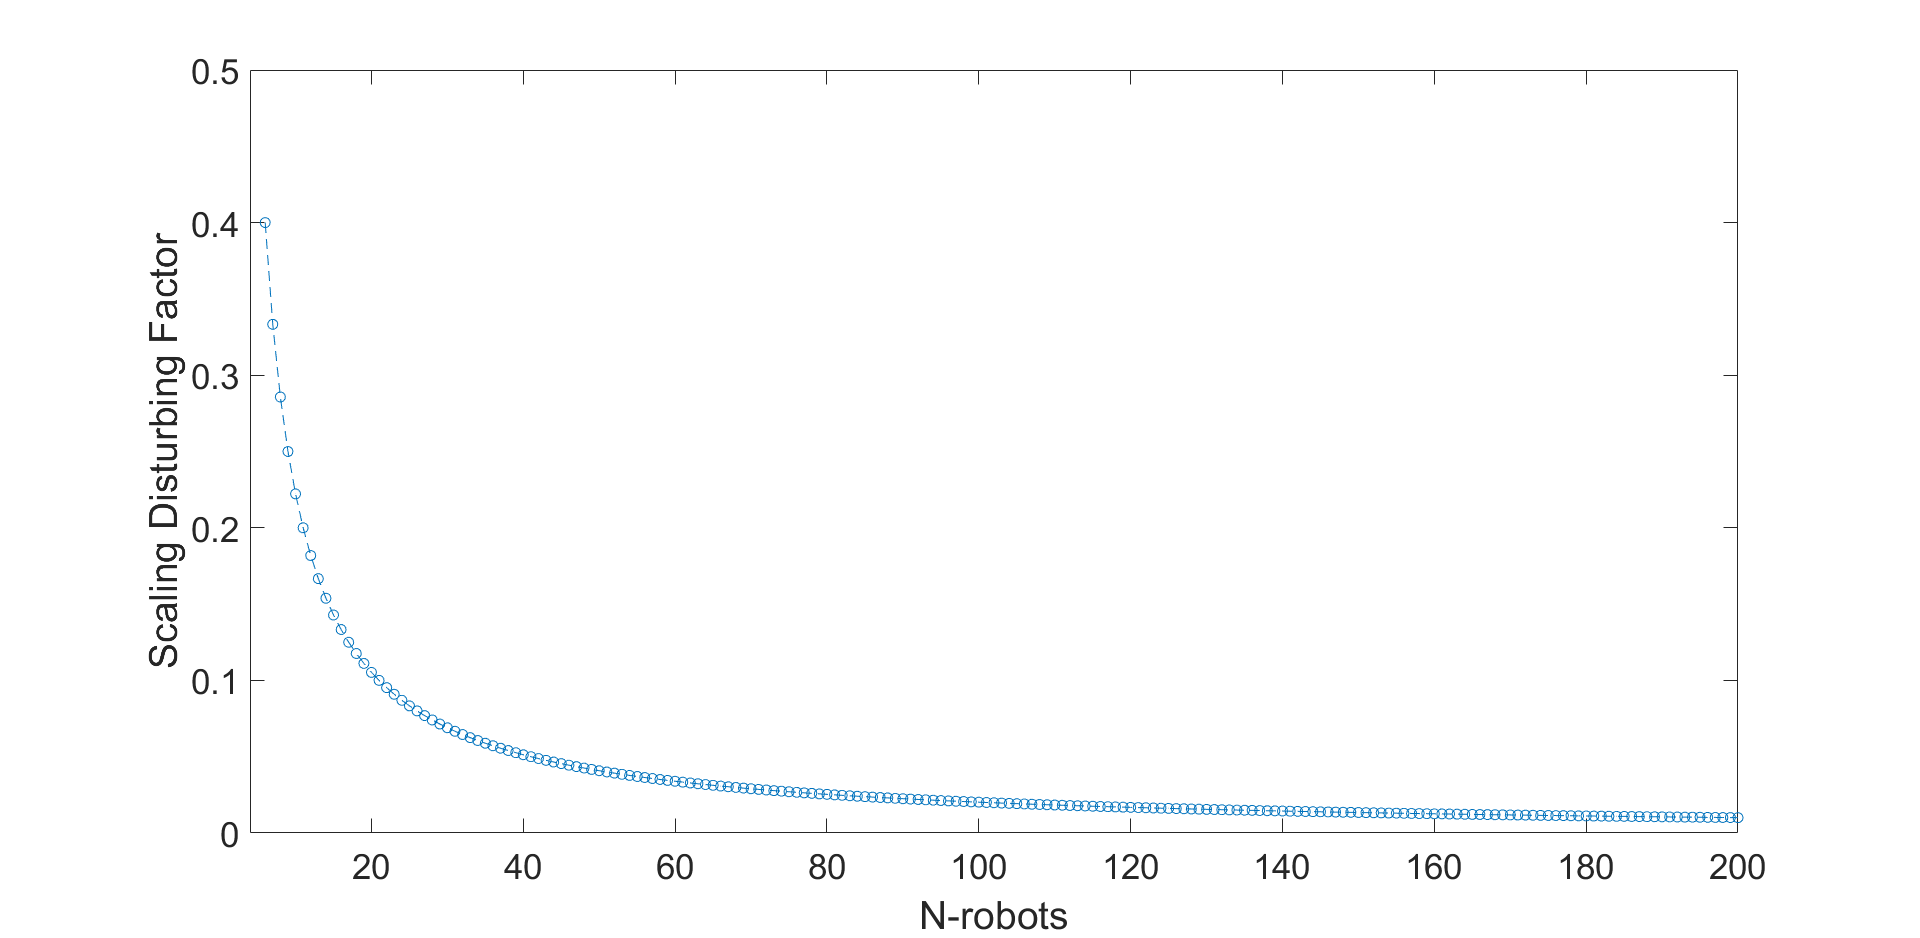
\includegraphics[width=1.1\textwidth]{figures/scalingFactorDisturbance.png}\\
\end{columns}

\end{frame}

%------------------------------------------------
\section{Proportional Force P-ANTS}
%------------------------------------------------
\subsection{P-ANTS Global}
\begin{frame}
\frametitle{P-ANTS Case}
Proportional force (P-ANTS) case deals with lifting and pulling the object on rolling devices \vspace{.3cm}
\begin{itemize}
\item Heavyweight objects\vspace{.3cm}
\item Dominant friction is the rolling friction of the wheel\vspace{.3cm}
\item Both global and local information studies
\end{itemize}
\end{frame}
%------------------------------------------------

\begin{frame}
\frametitle{P-ANTS Follower's Controller}
The consensus protocol commonly used for flocking
\begin{equation}\label{pants}
\dot{F}_i=\sum_{j \in N_i} (F_j - F_i)=\sum_{j \in N_i}F_j-NF_i
\end{equation}
\begin{itemize}
%\item $N_i$ is the interaction neighborhood
%\item $F_i$ is the force of the studied robot
\item $N$-complete graph
\end{itemize}
Employing equation \ref{roldyn} 
\begin{equation}\label{pantsdyn}
\dot{F}_i=M\dot{v}+\mu_v v-NF_i
\end{equation} 
\begin{itemize}
\item Reach consensus while the leader does not change its force
\item $\dot{v}$, $v$ object's velocity and acceleration at the CoM
\end{itemize}
\end{frame}
%------------------------------------------------

\begin{frame}
\frametitle{P-ANTS State Equations}
The state equations of P-ANTS
\begin{equation}
\dot{\eta}=-\eta+F_l
\end{equation}
\begin{equation}
F_s=(N-1)\eta+F_l
\end{equation}
\begin{itemize}
\item $F_l$, leader's force and the input
\item $\eta=(\sum_{i=2}^{N}F_i)/(N-1)$, avg force of the followers and state
\item $F_s=\sum_{i=1}^N F_i$, total force and the output of our system
\end{itemize}
\end{frame}

%------------------------------------------------

\subsection{P-ANTS Local}
\begin{frame}
\frametitle{P-ANTS Local Follower's Controller}
Follower's force feedback controller using local measurements
\begin{equation}\label{pantsdlm}
\dot{F}_i=(\sum_{j \in N}F_j-NF_i)-\frac{M}{J}r_i\times (\sum_{j\in N}r_j\times F_j)
\end{equation}
\begin{itemize}
\item 1$^{st}$ term: Similar to equation \ref{pants}
\item 2$^{nd}$ term: Disturbing term, we want to eliminate 
\item Leader's torque assumed to be negligible for many robots
\item Under assumption 3 the centrifugal terms eliminated
\end{itemize}
\end{frame}

%------------------------------------------------

\begin{frame}
\frametitle{P-ANTS Local Follower's Controller Matrix Form}
The matrix form of follower's force feedback controller using local measurements
\begin{equation}\label{mpants}
\dot{F}=\Bigg( -L_a-\frac{M}{J}R_a(t) \Bigg)F = -LF
\end{equation}
\begin{itemize}
\item $F \in \mathbb{R}^{2N}$, vector of followers and leader forces
\item $R_a(t) \in \mathbb{R}^{2N\times 2N}$, product of skew matrices
\item The matrix form only focus on 2D-space
\end{itemize}
\end{frame}

%------------------------------------------------

\begin{frame}
\frametitle{P-ANTS Local Follower's Controller Boundary Condition}
Eigenvalues o Laplacian matrix are less or equal to zero only if 
\begin{equation}
\frac{M}{J}\sum_{i=1}^N||r_i||^2<N
\end{equation}
\begin{itemize}
\item Restricts the number of robots 
\begin{enumerate}
\item Object's mass $M$
\item Inertia matrix $J$
\item Radius from contact point to CoM of object $r_i$
\end{enumerate}
\end{itemize}
\end{frame}

%------------------------------------------------
\section{Simulations}
%------------------------------------------------
\begin{frame}
\frametitle{CB-ANTS Global}

Velocity direction alignment and force consensus in x and y axes

\begin{columns}[c] 
\column{.55\textwidth}
\centering
 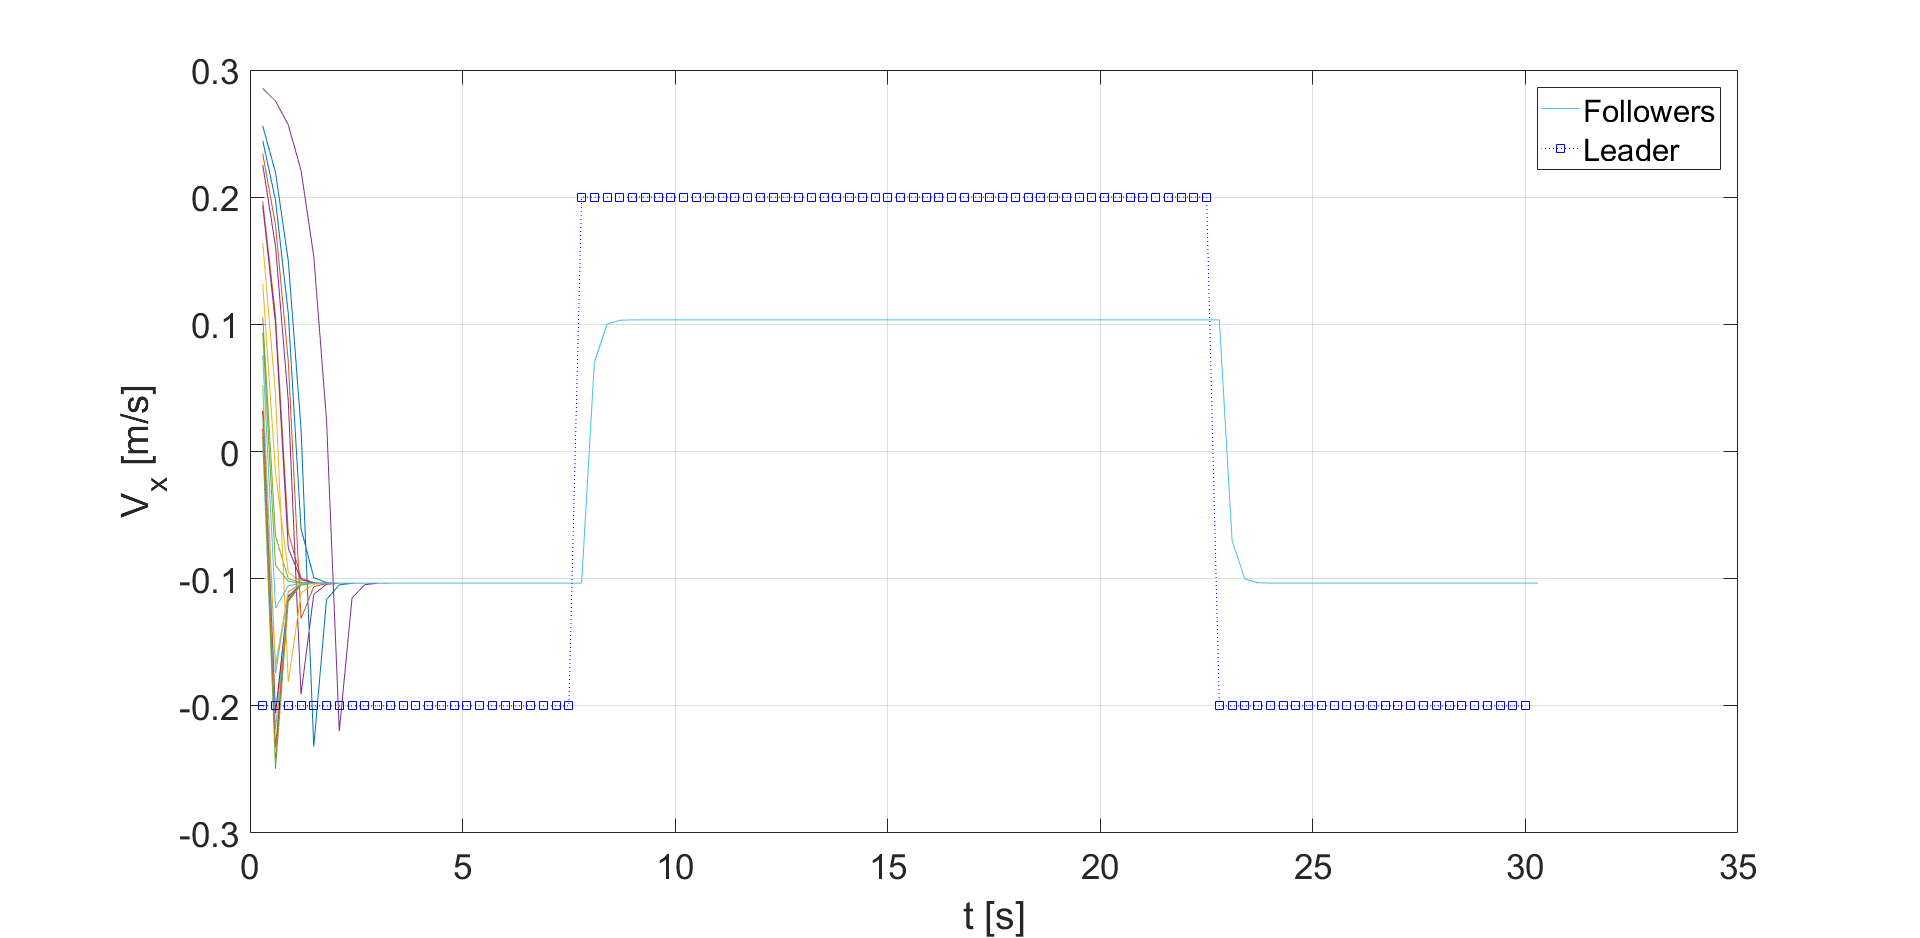
\includegraphics[width=1\textwidth]{figures/CB_ANTS_Vx.png}

\column{.55\textwidth} 
\centering
 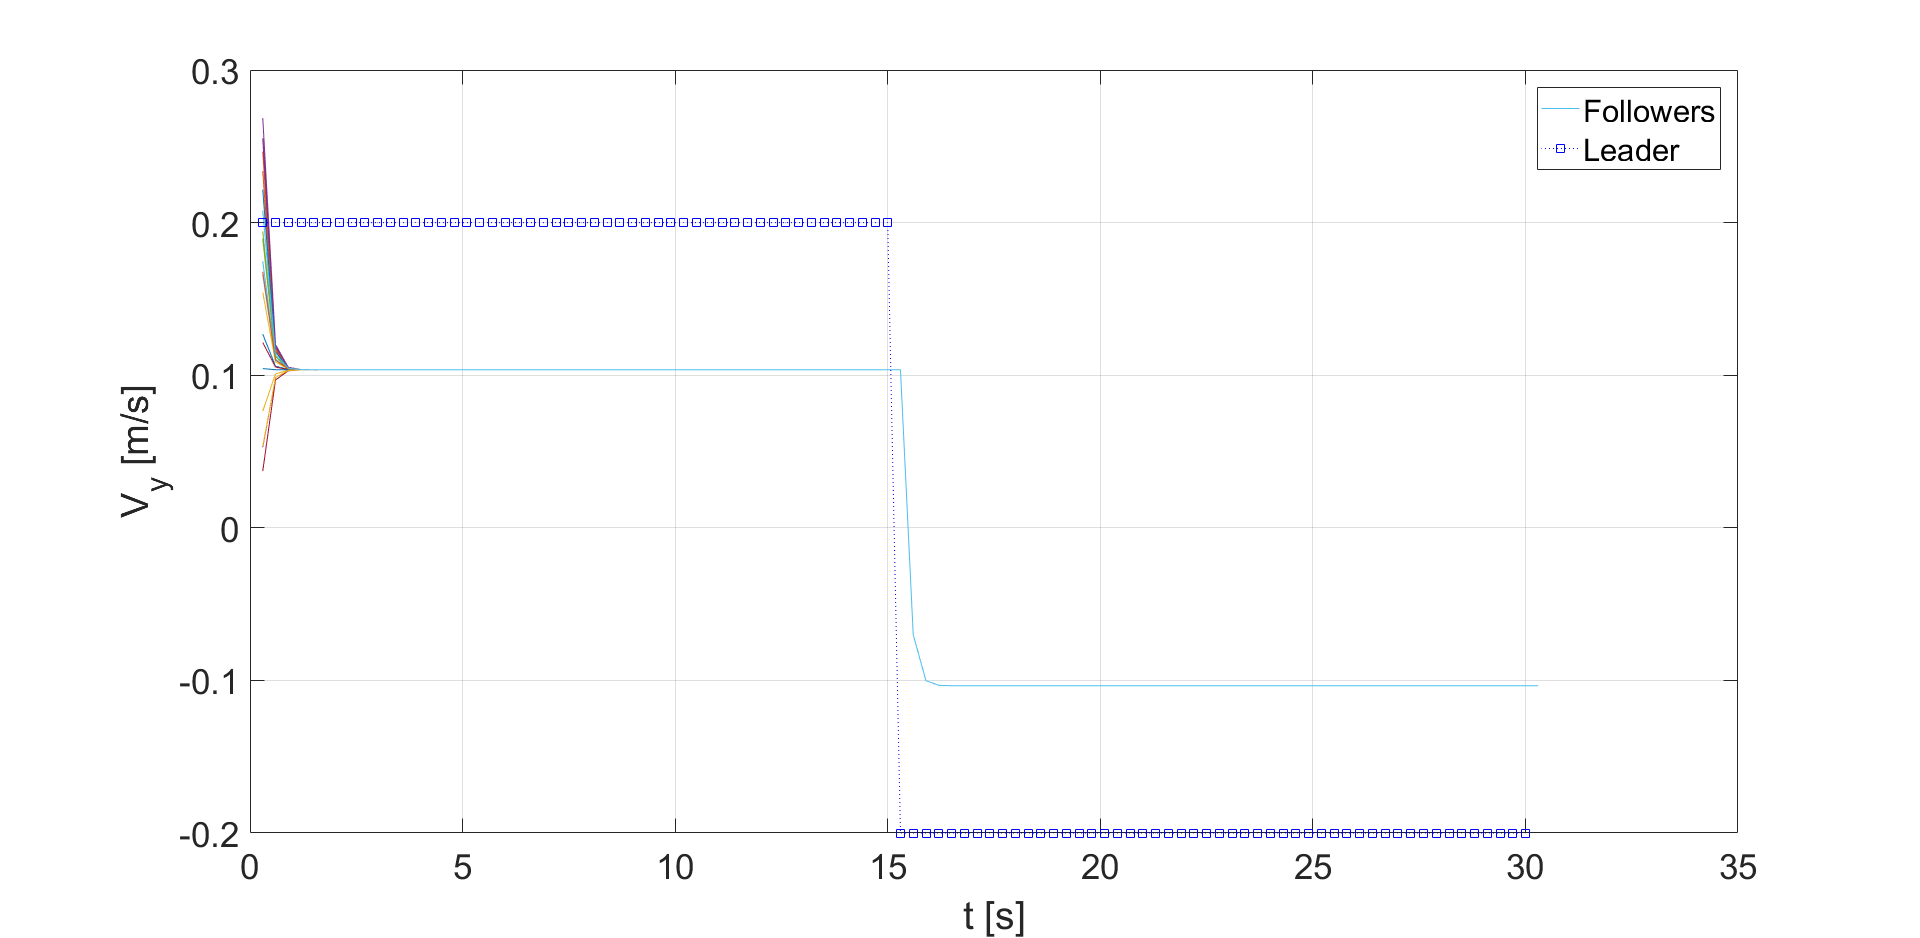
\includegraphics[width=1\textwidth]{figures/CB_ANTS_Vy.png}
\end{columns}

\begin{columns}[c] 
\column{.55\textwidth}
\centering
 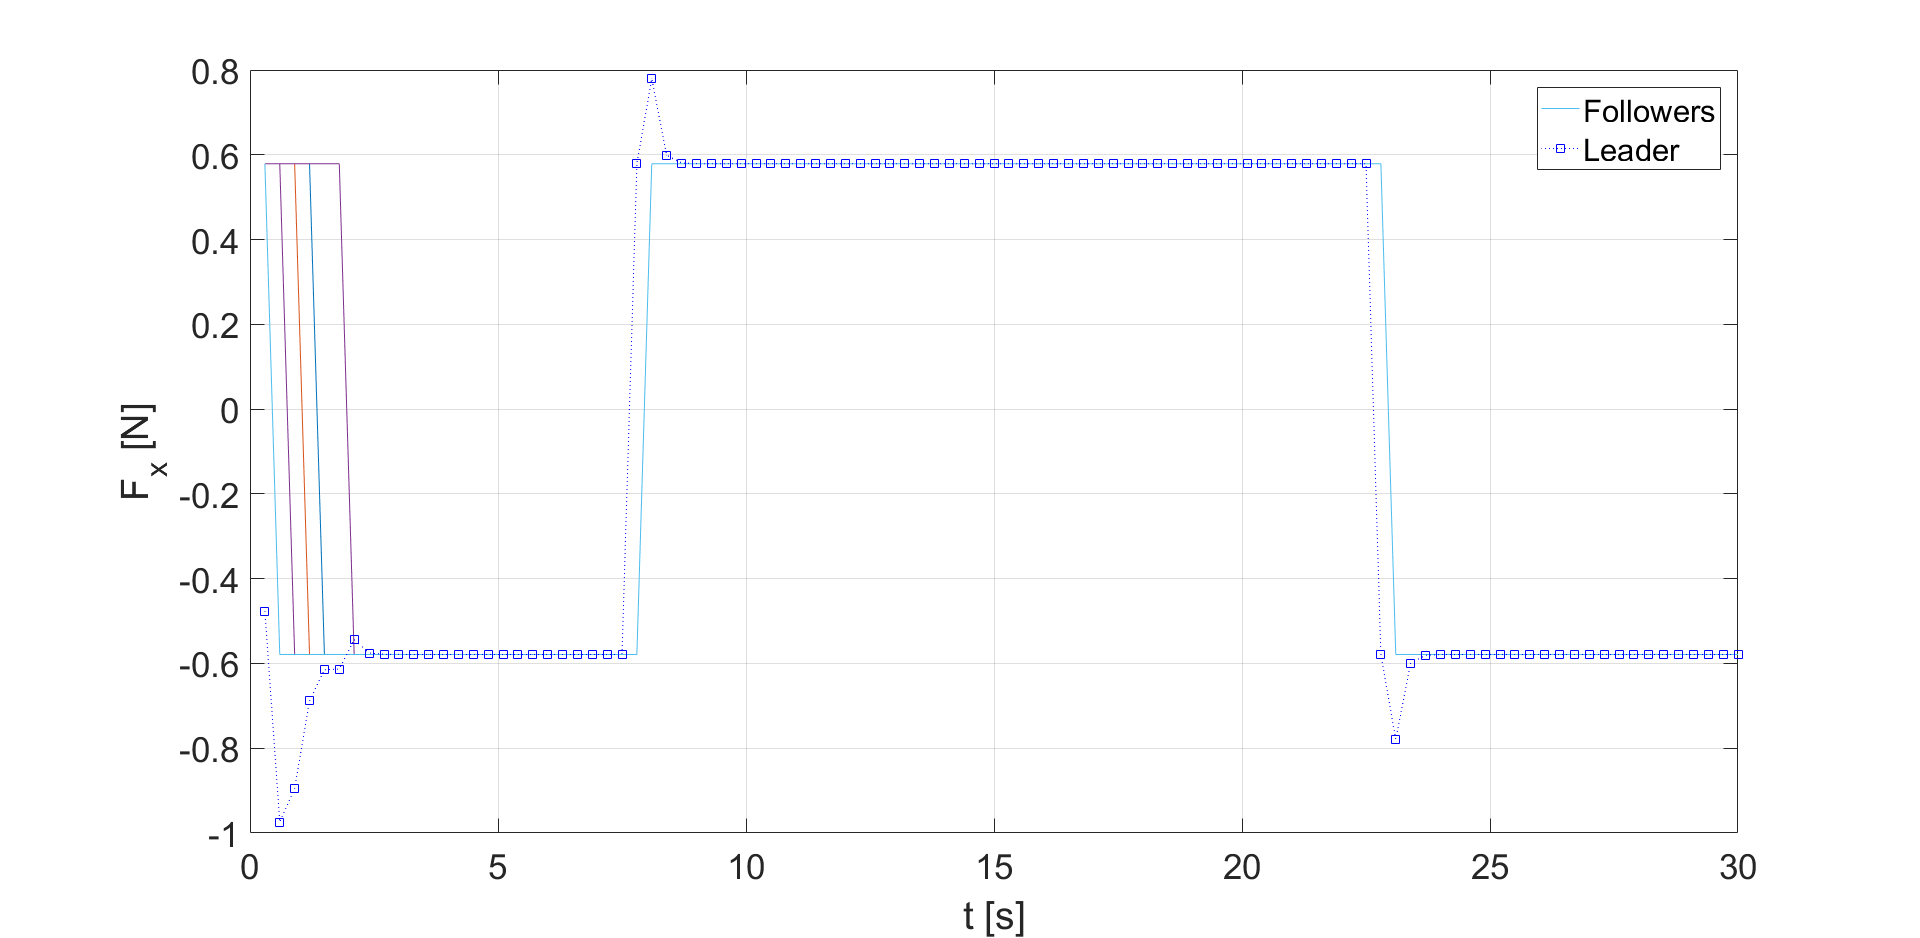
\includegraphics[width=1\textwidth]{figures/CB_ANTS_Fx.png}

\column{.55\textwidth} 
\centering
 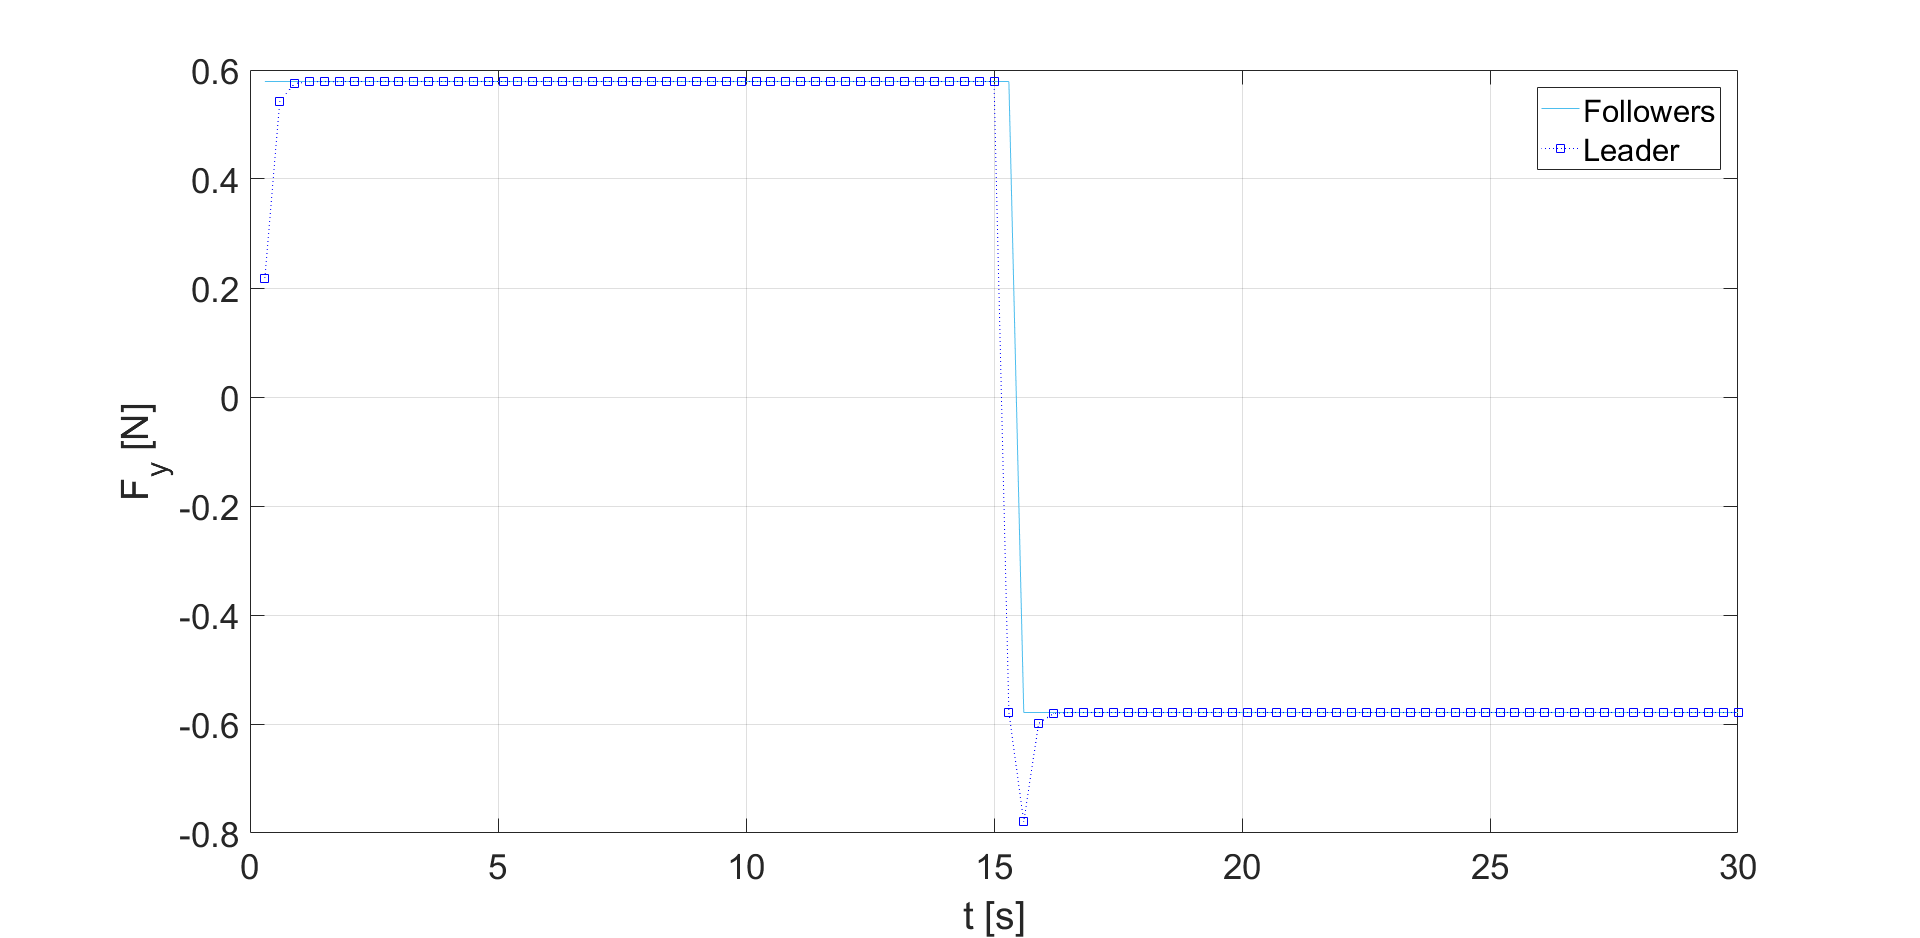
\includegraphics[width=1\textwidth]{figures/CB_ANTS_Fy.png}
\end{columns}

\end{frame}

%------------------------------------------------

\begin{frame}
\frametitle{P-ANTS Global}

Sum of forces and force consensus in x and y axes

\begin{columns}[c] 
\column{.55\textwidth}
\centering
 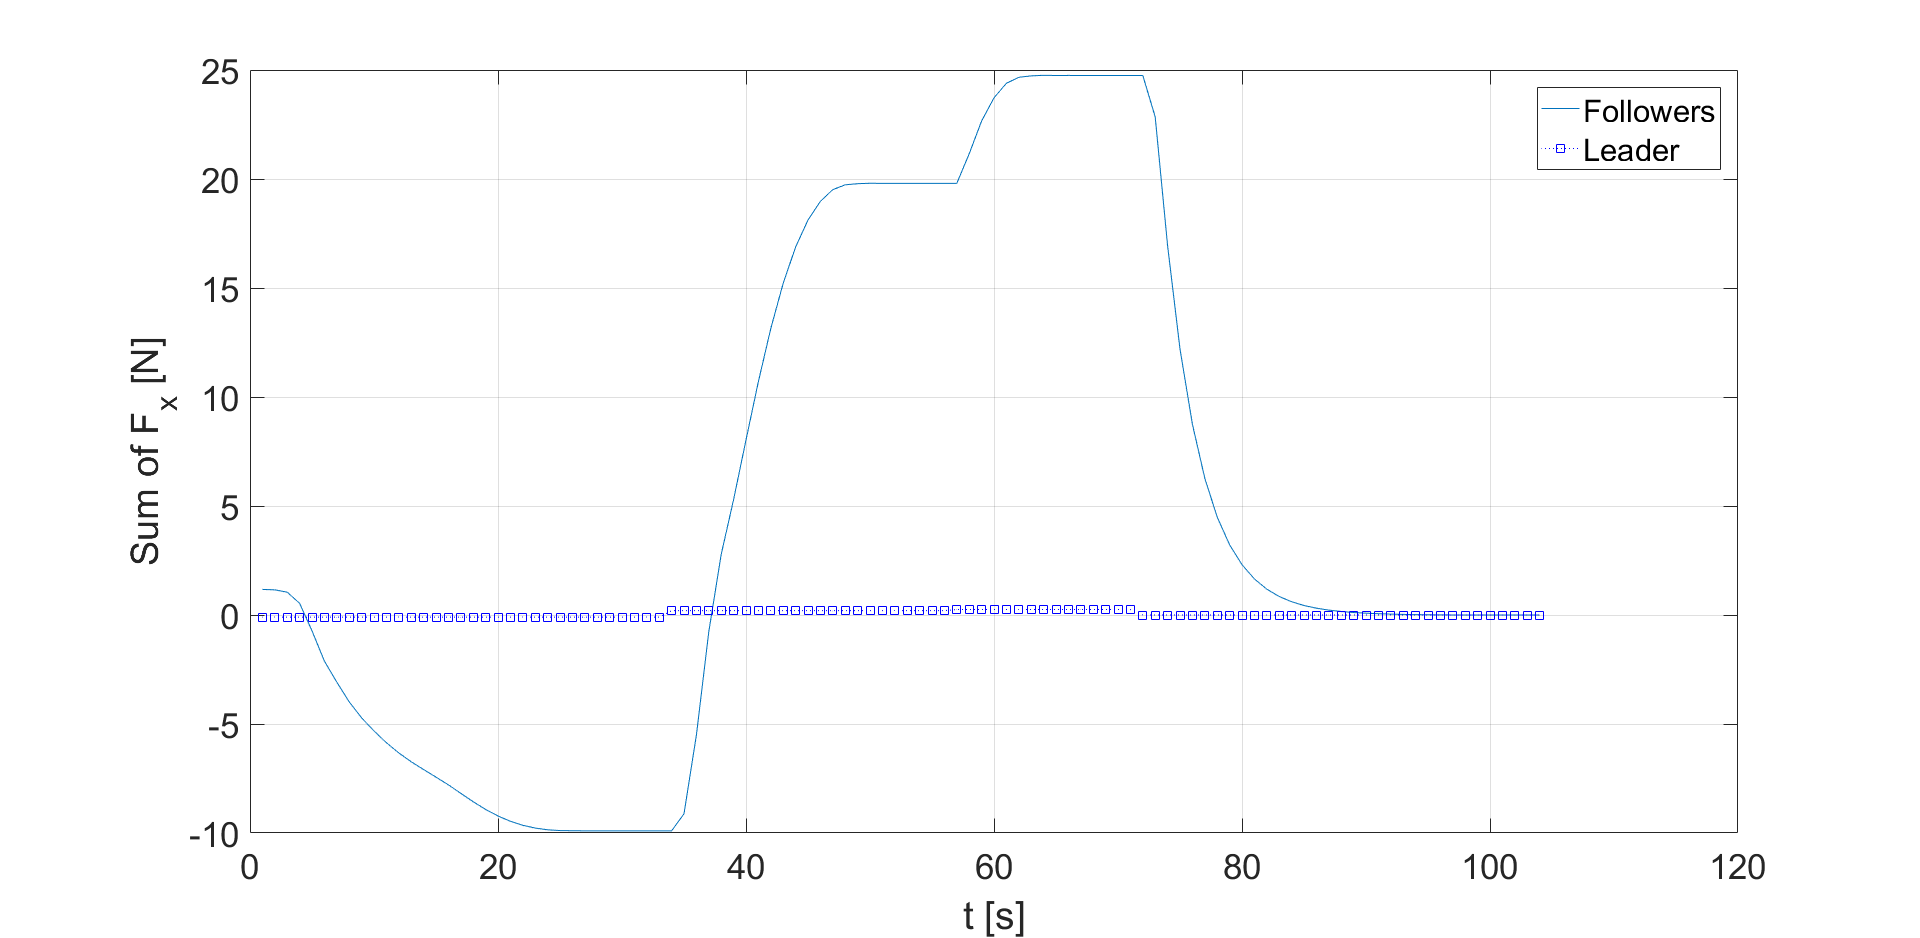
\includegraphics[width=1\textwidth]{figures/P_ANTS_SumFx.png}

\column{.55\textwidth} 
\centering
 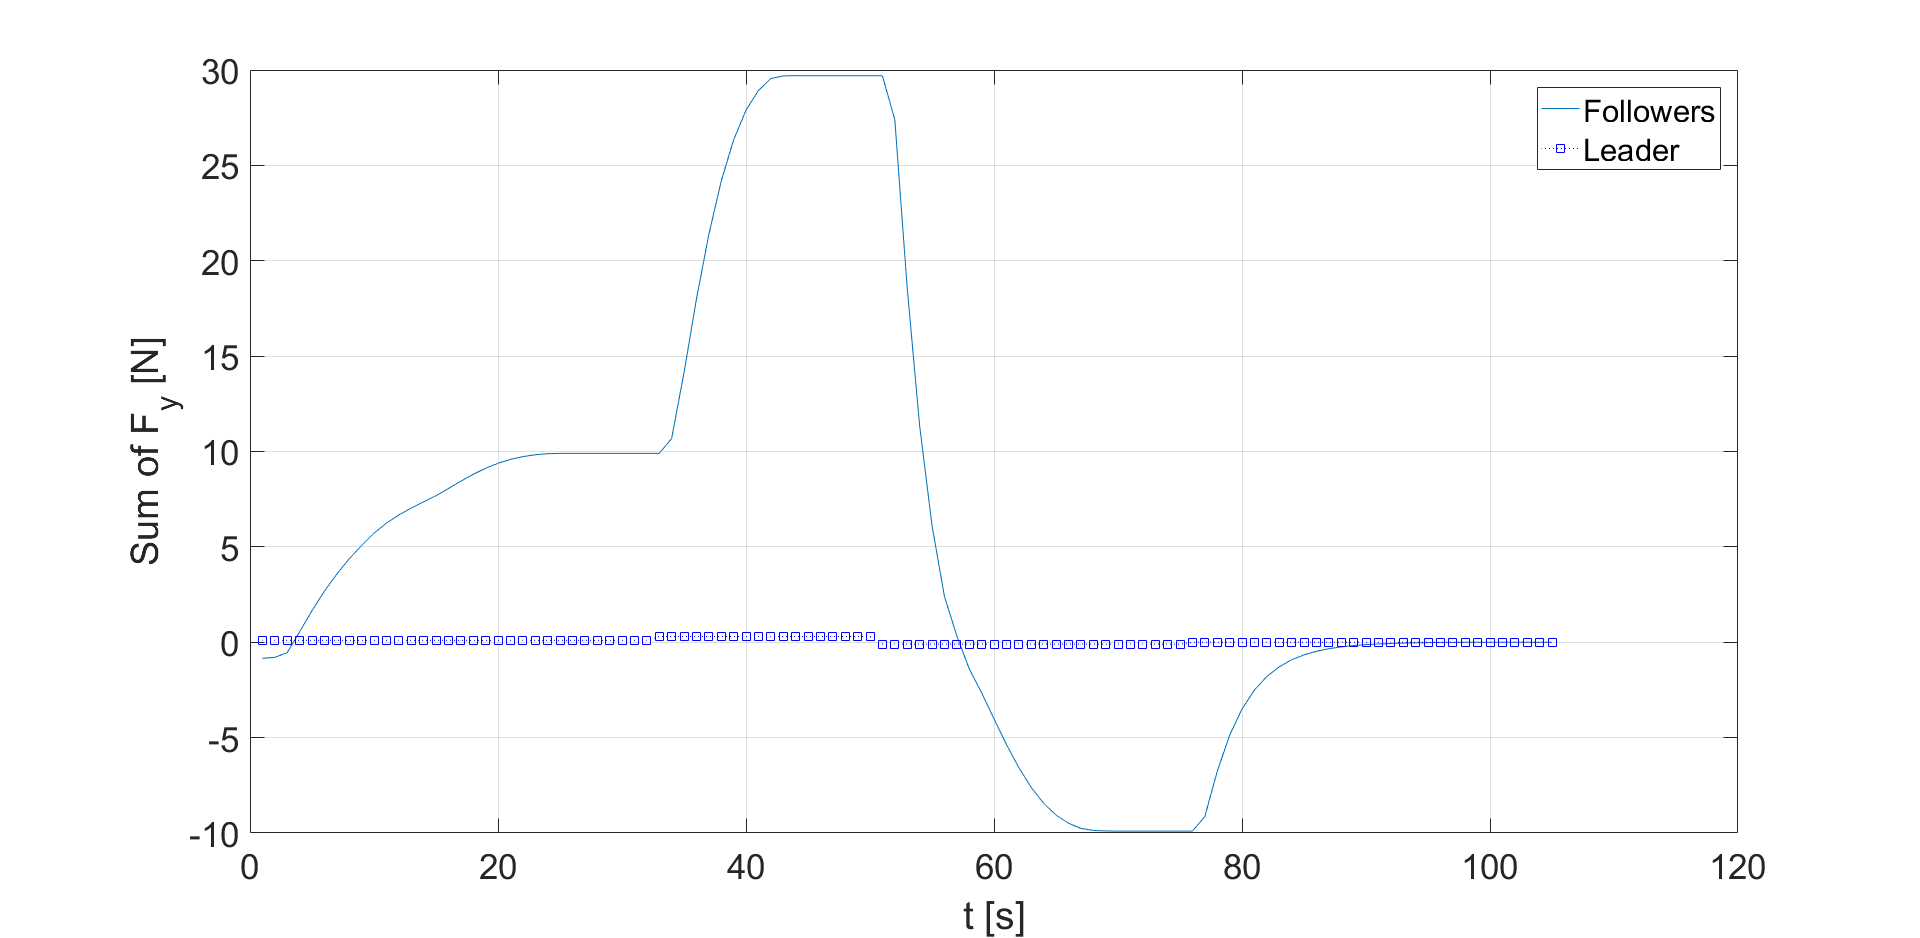
\includegraphics[width=1\textwidth]{figures/P_ANTS_SumFy.png}
\end{columns}

\begin{columns}[c] 
\column{.55\textwidth}
\centering
 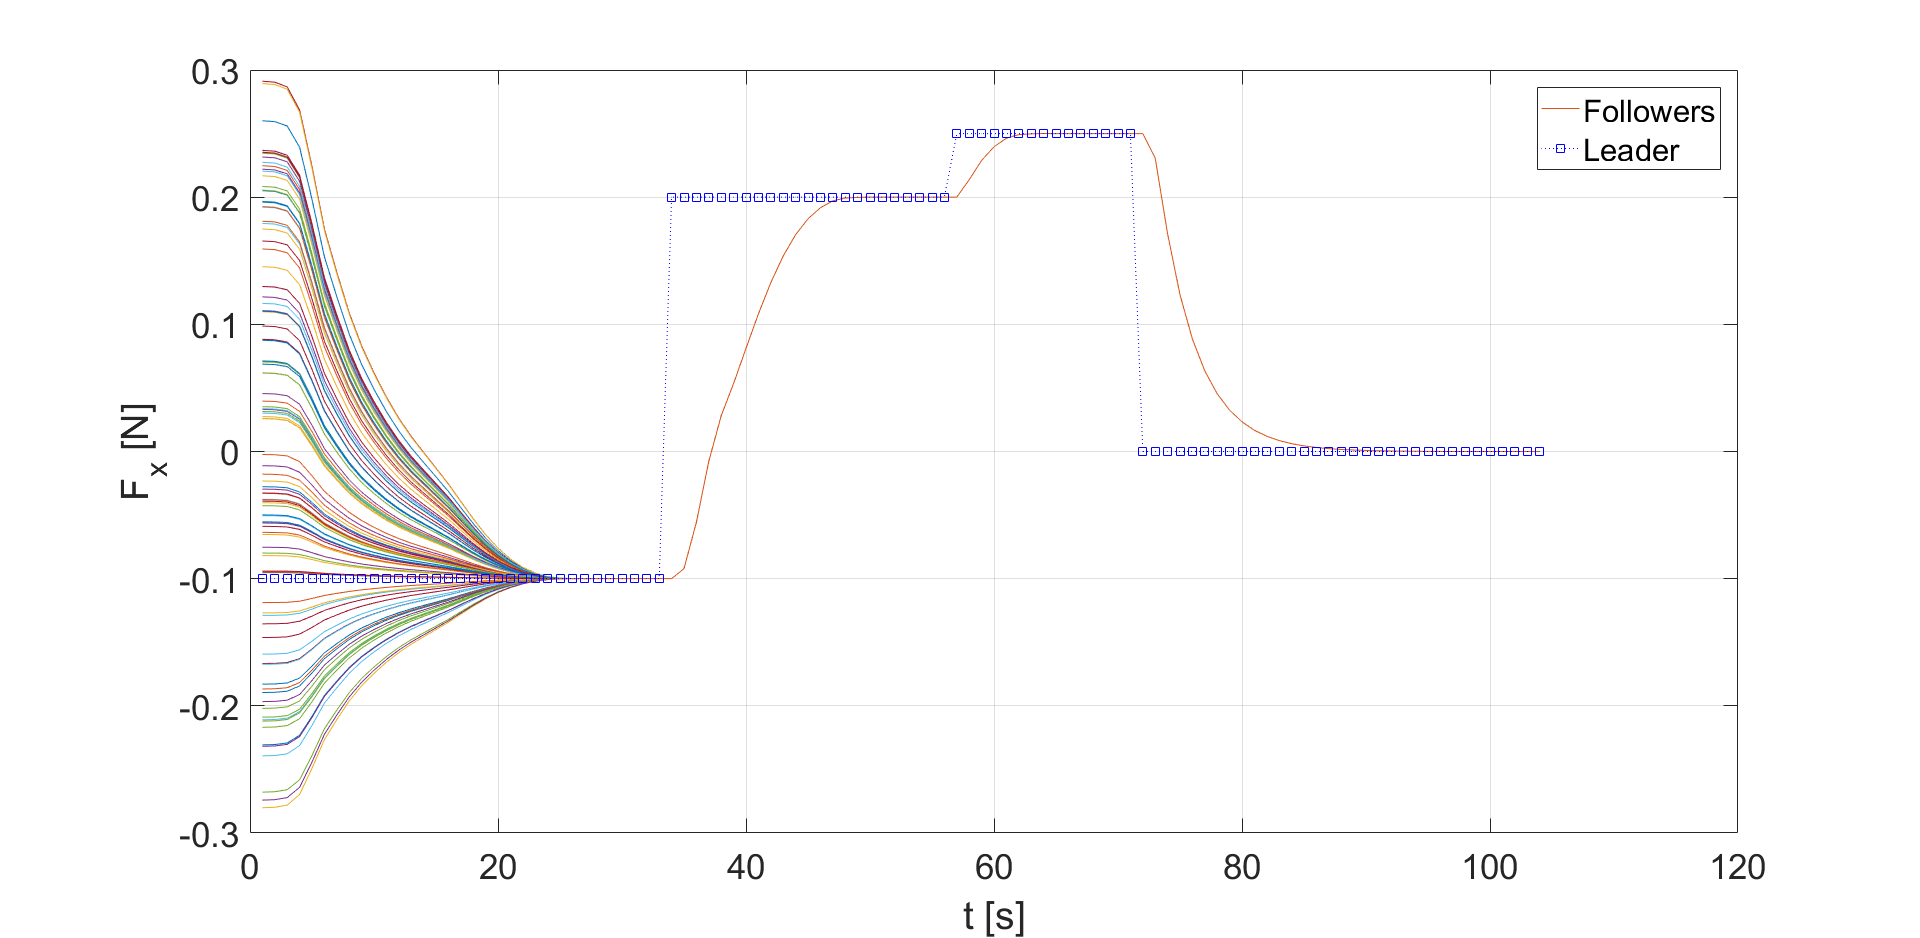
\includegraphics[width=1\textwidth]{figures/P_ANTS_Fx.png}

\column{.55\textwidth} 
\centering
 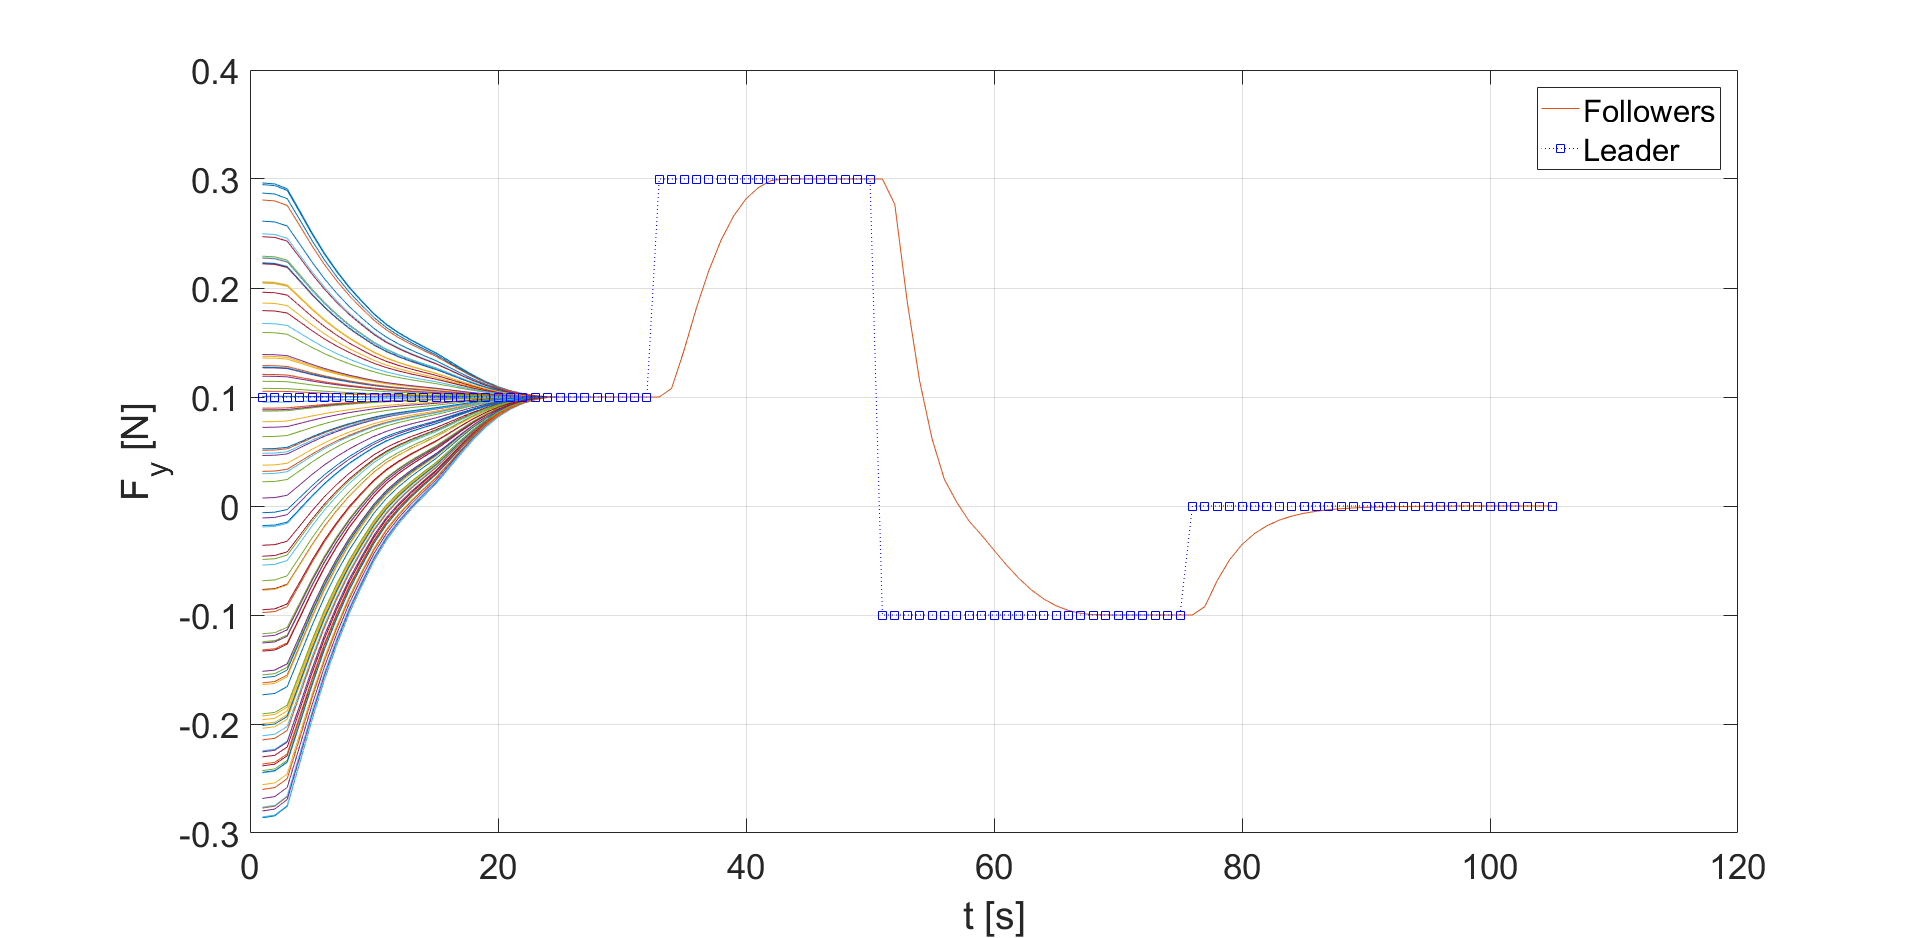
\includegraphics[width=1\textwidth]{figures/P_ANTS_Fy.png}
\end{columns}

\end{frame}

%------------------------------------------------

\begin{frame}
\frametitle{P-ANTS Local}

Force consensus w/ 10 and 100 robots in x and y axes

\begin{columns}[c] 
\column{.55\textwidth}
\centering
 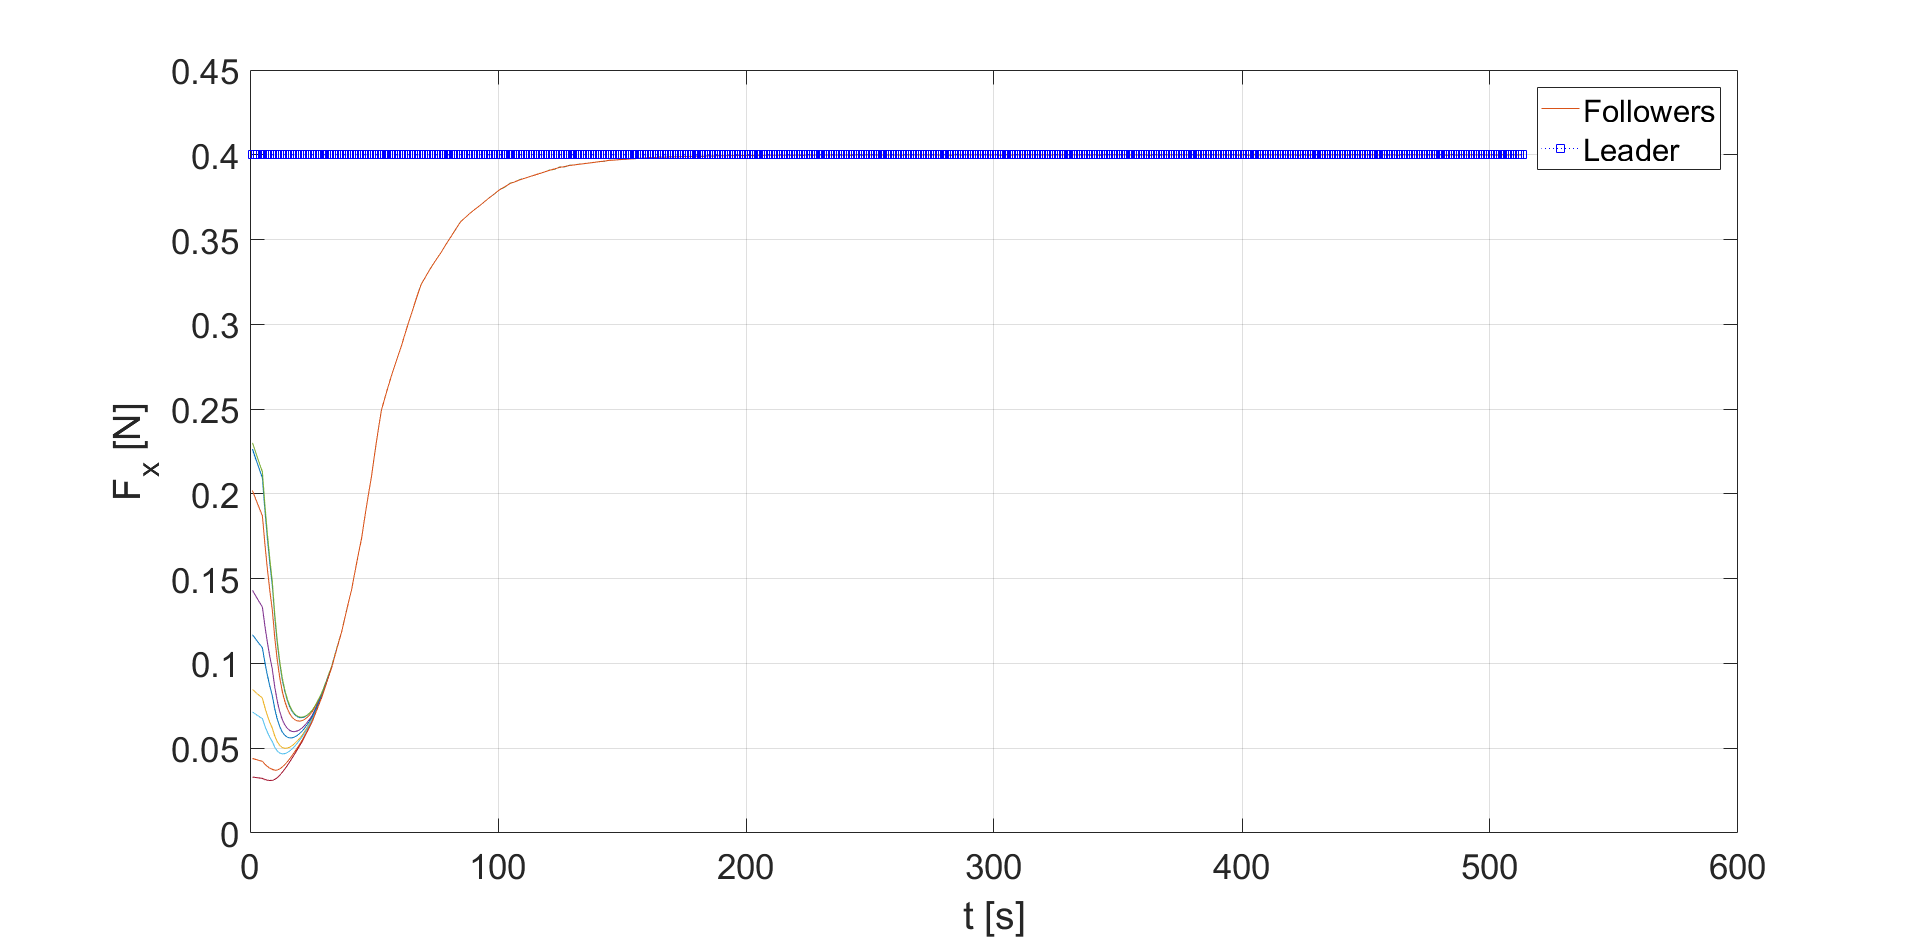
\includegraphics[width=1\textwidth]{figures/P_ANTS_Local_Fx.png}

\column{.55\textwidth} 
\centering
 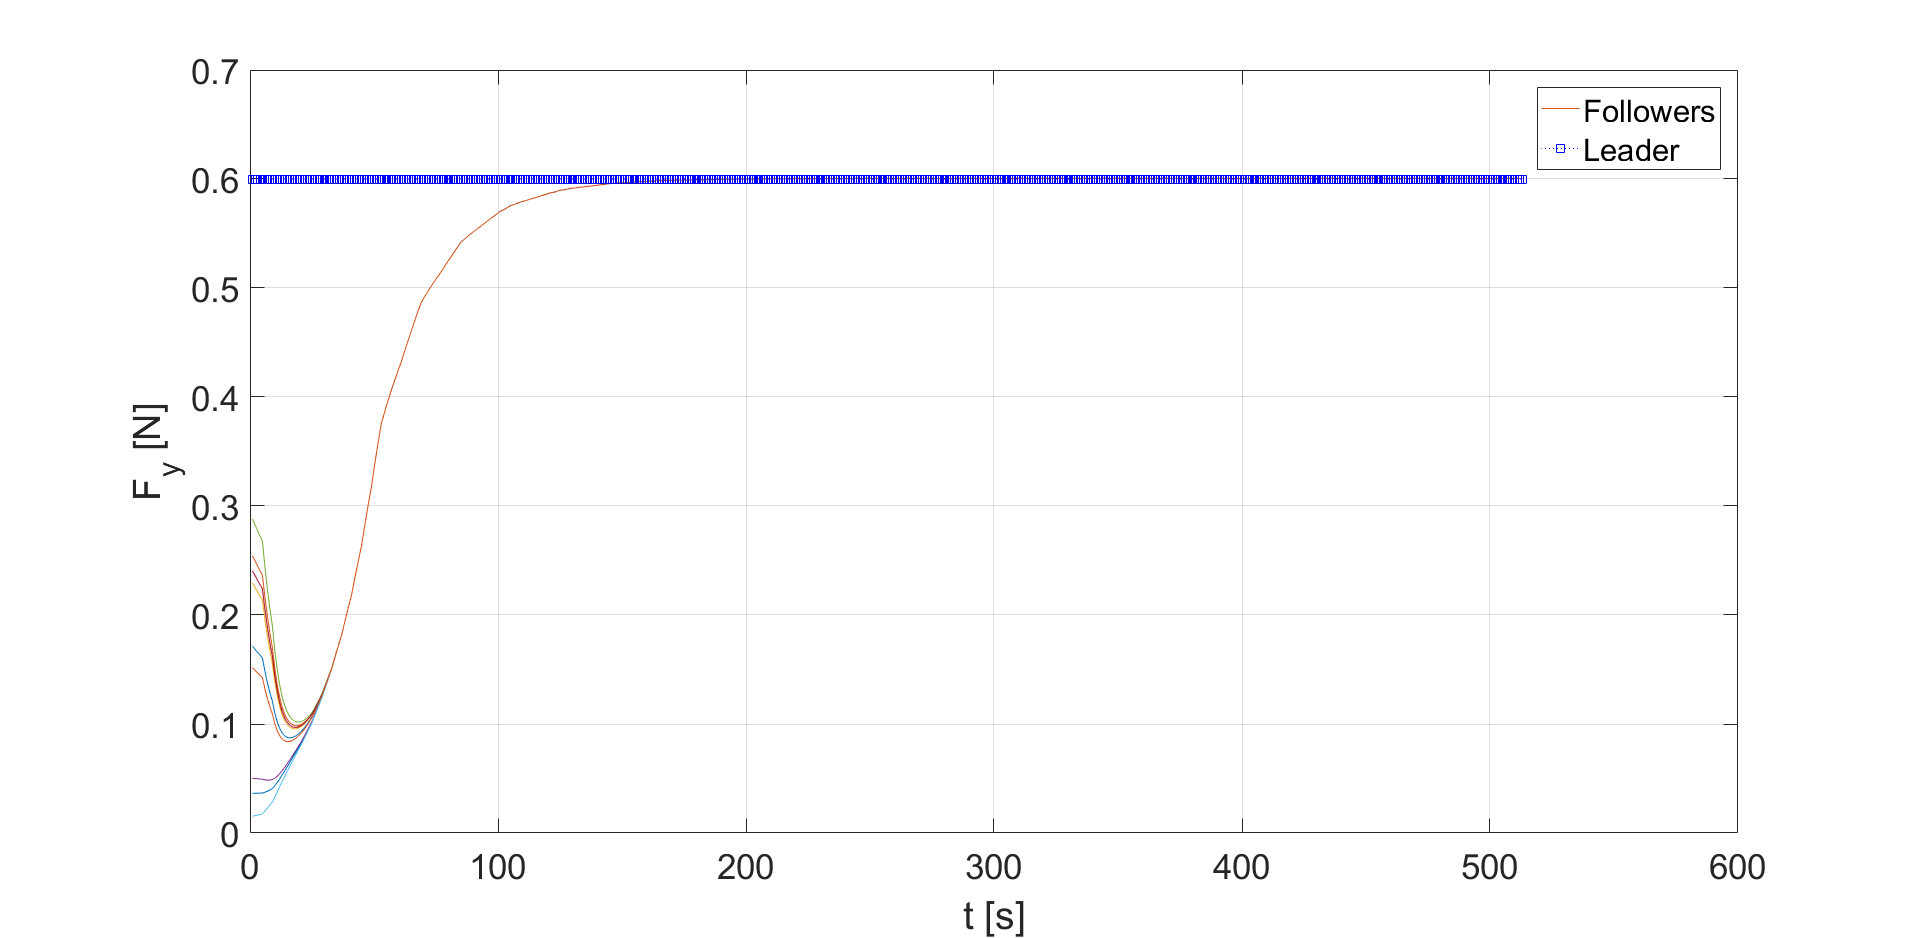
\includegraphics[width=1\textwidth]{figures/P_ANTS_Local_Fy.png}
\end{columns}

\begin{columns}[c] 
\column{.55\textwidth}
\centering
 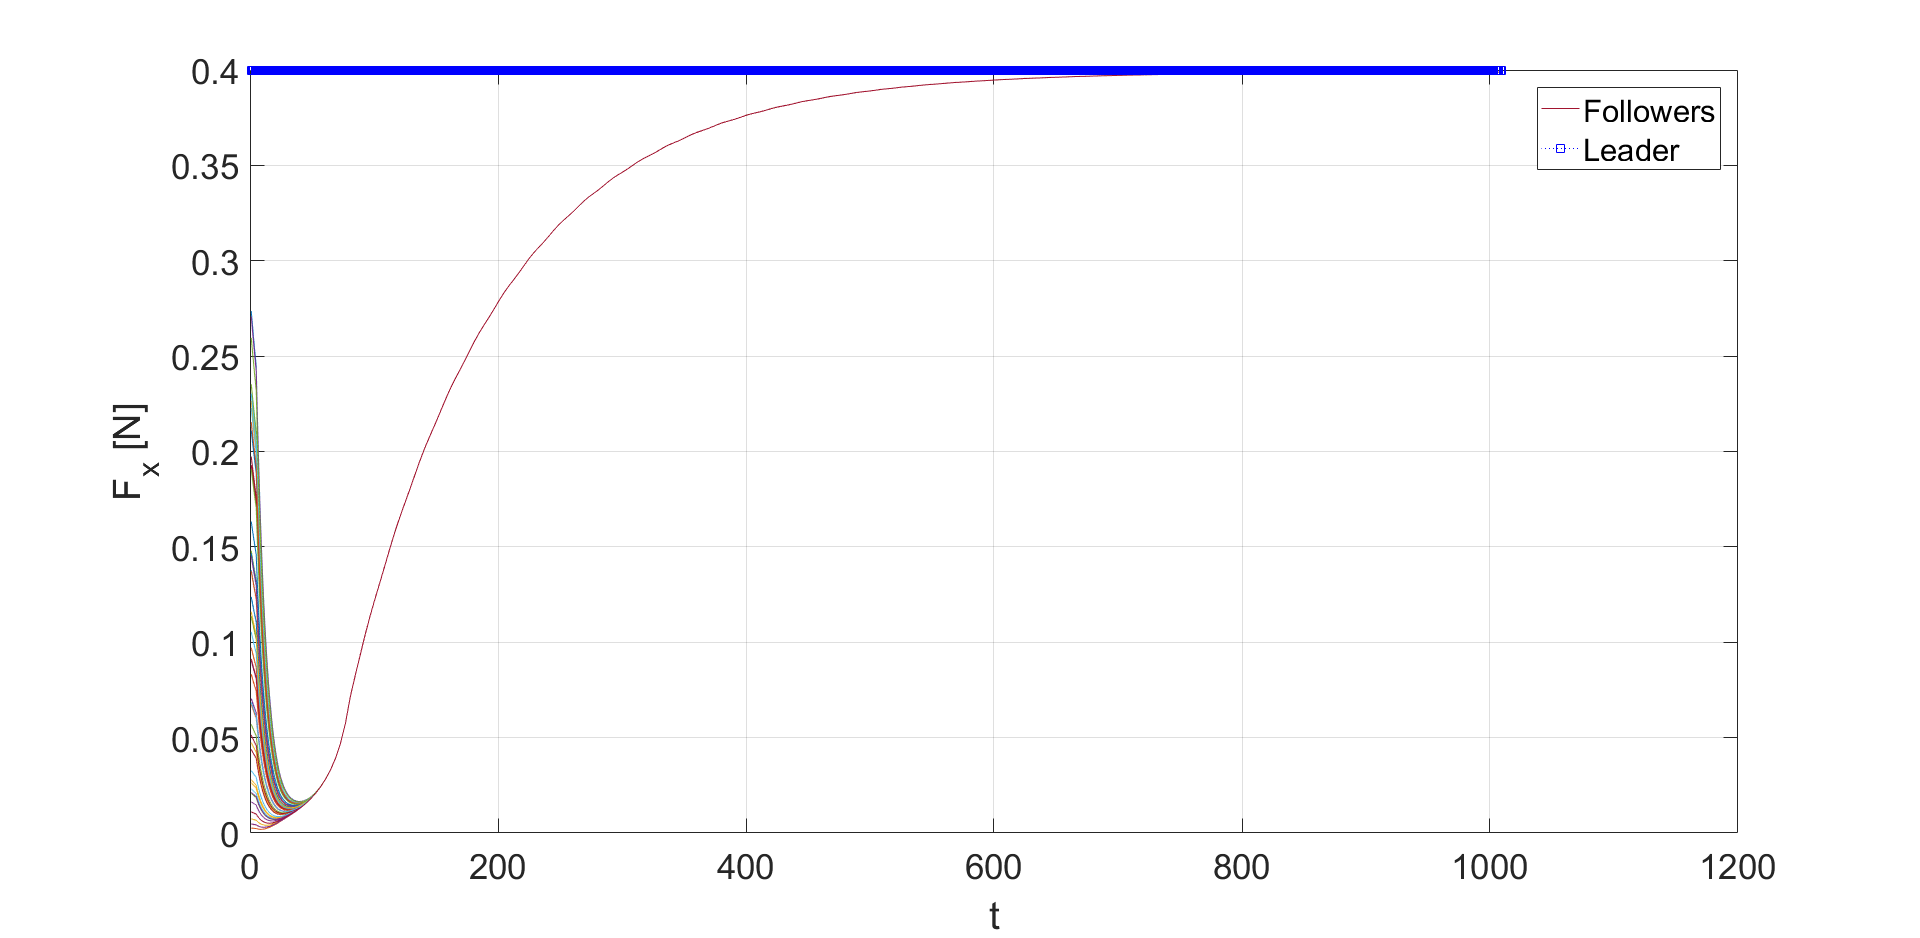
\includegraphics[width=1\textwidth]{figures/P_ANTS_Local_Fx_100.png}

\column{.55\textwidth} 
\centering
 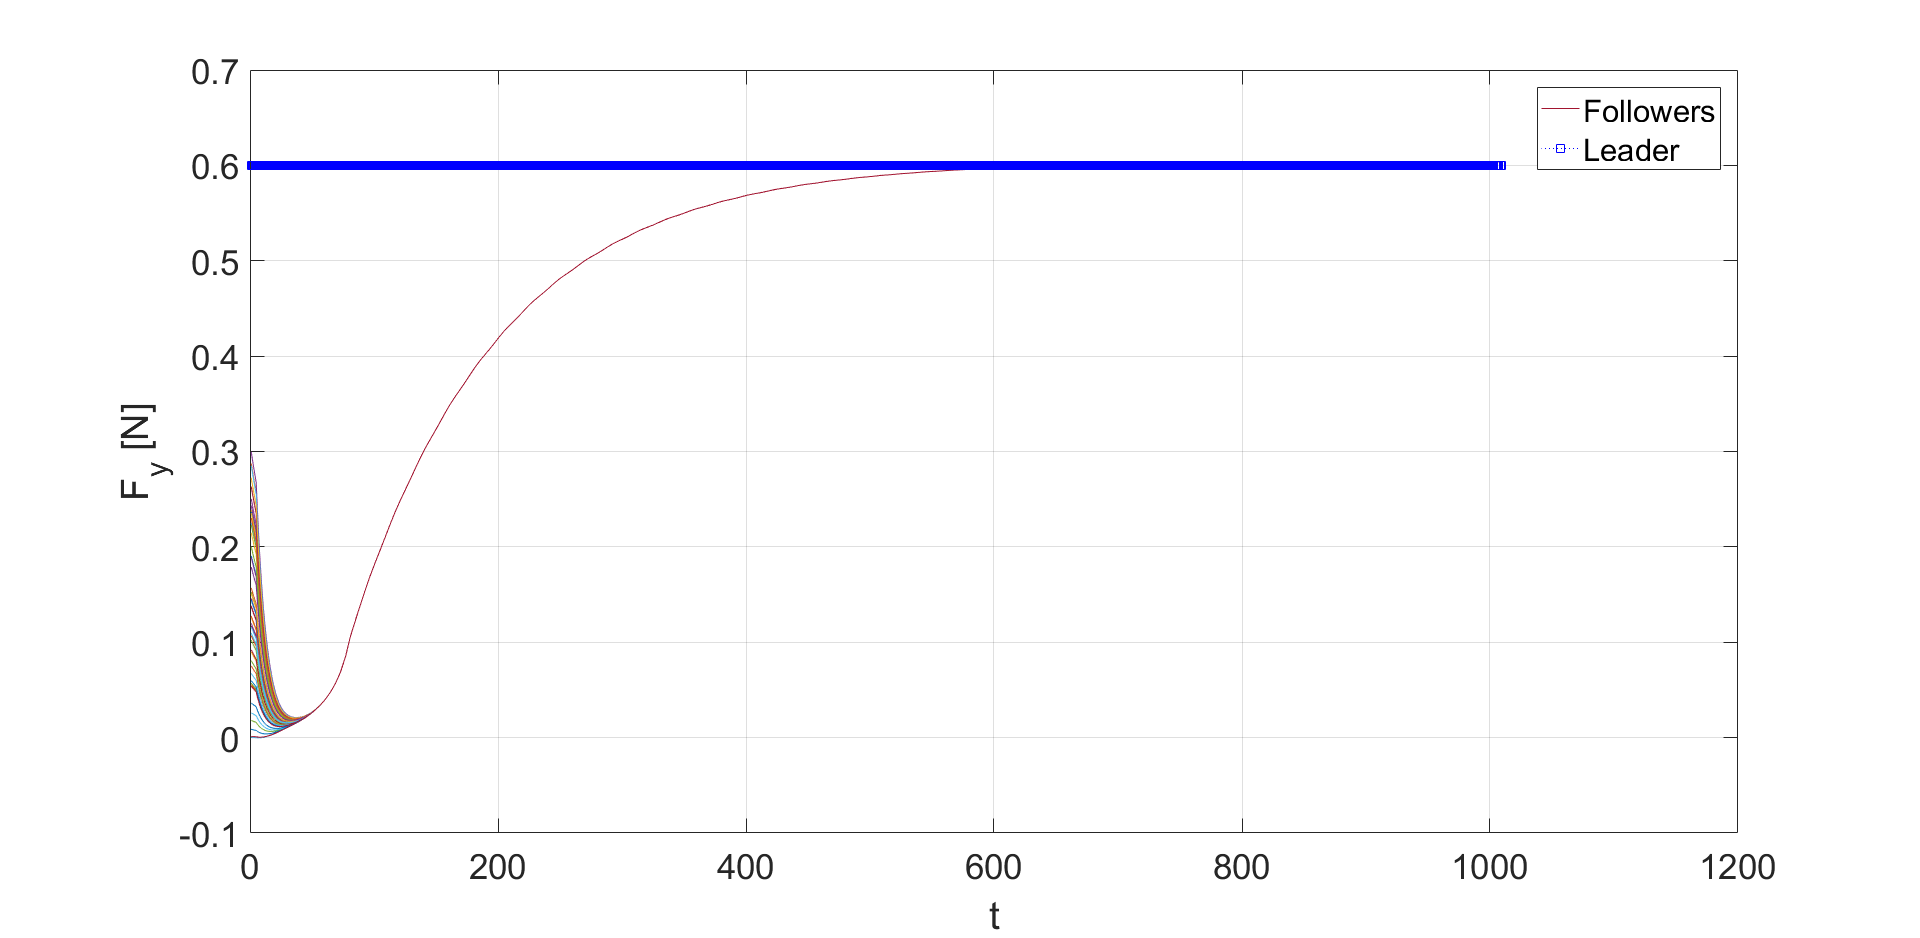
\includegraphics[width=1\textwidth]{figures/P_ANTS_Local_Fy_100.png}
\end{columns}

\end{frame}

%------------------------------------------------

\section{Conclusions}
\begin{frame}
\frametitle{Conclusions}
\begin{itemize}
\item Cooperative manipulation framework w/o explicit communication presented\vspace{.2cm}
\item Force feedback information utilized \vspace{.2cm}
\item Leader robot impose its force intention to the followers \vspace{.2cm}
\item Two different cases studied depending on the object weight 
\begin{itemize}
\item CB-ANTS for lightweight objects by dragging
\item P-ANTS for heavyweight objects by lifting and pulling on rolling devices\vspace{.2cm}
\end{itemize}
\item Two solutions presented for each case
\begin{itemize}
\item Using global measurements
\item Using local measurements
\end{itemize}
\end{itemize}
\end{frame}


%------------------------------------------------
\begin{frame}
\frametitle{Random Thoughts}
\begin{itemize}
\item Discretization of object's dynamics\vspace{.2cm}
\item Assumption 1, 2, 3 make the methodology compatible only in structured environments\vspace{.2cm}
\item Assumption 3 for CB-ANTS and small number of robots is not feasible\vspace{.2cm}
%\item Could not implement CB-ANTS w/ local measurements\vspace{.2cm}
\item State equations for P-ANTS should not be used, because they are based on $N$-Complete graph \vspace{.2cm}
\item P-ANTS w/ local measurements should extend in 3$D$-space, because the inertia matrix is affected\vspace{.2cm}
\end{itemize}
\end{frame}







%------------------------------------------------
\section{References}
%------------------------------------------------

\begin{frame}
\frametitle{References}
\tiny{
\begin{thebibliography}{99} % Beamer does not support BibTeX so references must be inserted manually as below


\bibitem[Wang, 2016]{p1} Z. Wang, M. Schwager
\newblock Force-Amplifying N-Robot Transport System (Force-ANTS) for Cooperative Planar Manipulation without Communication
\newblock \emph{International Journal of Robotics Research, 1564--1586, SAGE Publications}, 2016.

\bibitem[Wang, 2015]{p2} Z. Wang, M. Schwager
\newblock Multi-robot manipulation with no communication using only local measurements
\newblock \emph{54th Annual Conference on Decision and Control (CDC), 380--385, IEEE}, 2015.

\bibitem[Wang, 2014]{p3} Z. Wang, M. Schwager
\newblock Multi-robot manipulation without communication
\newblock \emph{Distributed Autonomous Robotic Systems, 135--149, Springer}, 2014.

\bibitem[Wang, 2016]{p4} Z. Wang, M. Schwager
\newblock Kinematic multi-robot manipulation with no communication using force feedback
\newblock \emph{International Conference on Robotics and Automation (ICRA), 427--432, IEEE}, 2016.


\end{thebibliography}
}
\end{frame}

%------------------------------------------------
\section{}
\begin{frame}
\begin{center}
\Huge {Thank You!}
\end{center}
\end{frame}

%----------------------------------------------------------------------------------------

\end{document} 